
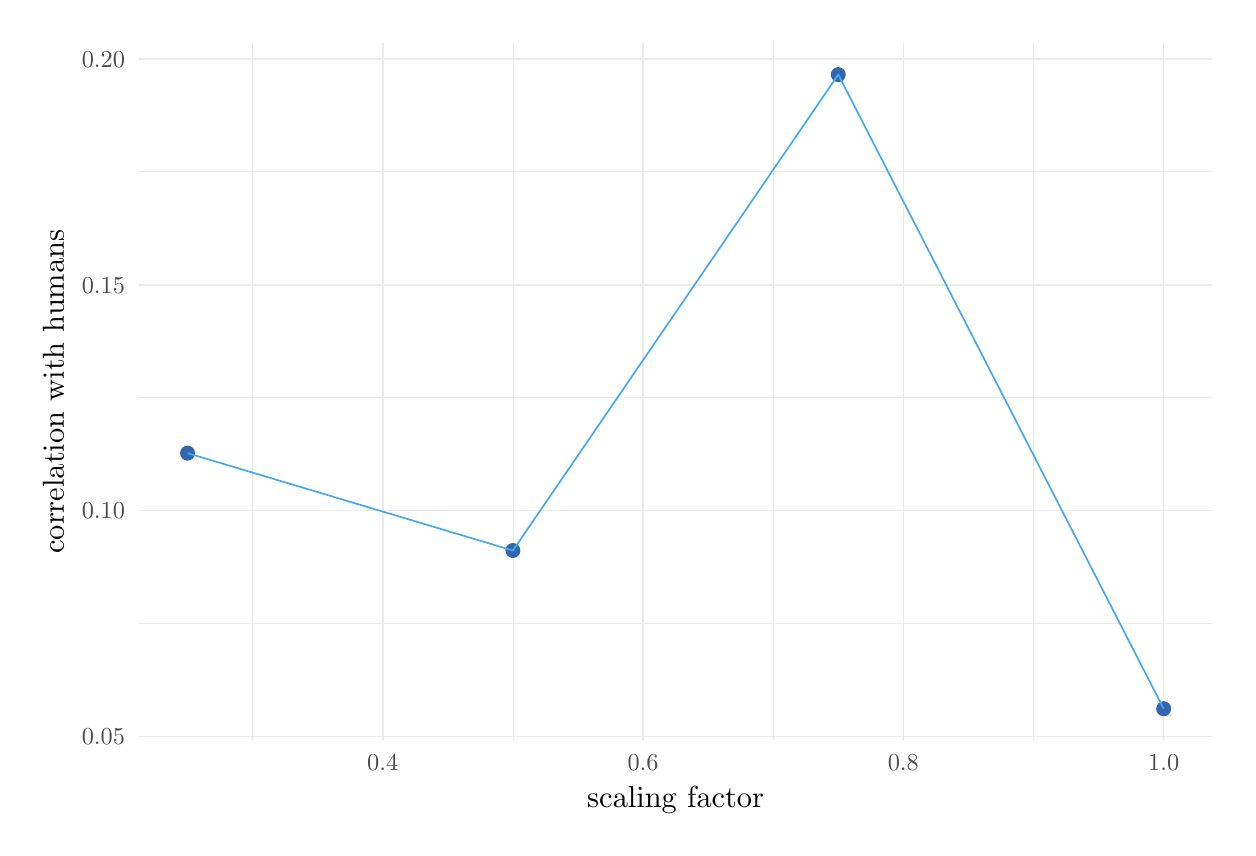
\begin{tikzpicture}[x=1pt,y=1pt]
\definecolor{fillColor}{RGB}{255,255,255}
\path[use as bounding box,fill=fillColor,fill opacity=0.00] (0,0) rectangle (433.62,289.08);
\begin{scope}
\path[clip] ( 40.14, 31.53) rectangle (428.12,283.58);
\definecolor{drawColor}{gray}{0.92}

\path[draw=drawColor,line width= 0.3pt,line join=round] ( 40.14, 73.78) --
	(428.12, 73.78);

\path[draw=drawColor,line width= 0.3pt,line join=round] ( 40.14,155.37) --
	(428.12,155.37);

\path[draw=drawColor,line width= 0.3pt,line join=round] ( 40.14,236.97) --
	(428.12,236.97);

\path[draw=drawColor,line width= 0.3pt,line join=round] ( 81.29, 31.53) --
	( 81.29,283.58);

\path[draw=drawColor,line width= 0.3pt,line join=round] (175.34, 31.53) --
	(175.34,283.58);

\path[draw=drawColor,line width= 0.3pt,line join=round] (269.40, 31.53) --
	(269.40,283.58);

\path[draw=drawColor,line width= 0.3pt,line join=round] (363.46, 31.53) --
	(363.46,283.58);

\path[draw=drawColor,line width= 0.6pt,line join=round] ( 40.14, 32.98) --
	(428.12, 32.98);

\path[draw=drawColor,line width= 0.6pt,line join=round] ( 40.14,114.58) --
	(428.12,114.58);

\path[draw=drawColor,line width= 0.6pt,line join=round] ( 40.14,196.17) --
	(428.12,196.17);

\path[draw=drawColor,line width= 0.6pt,line join=round] ( 40.14,277.76) --
	(428.12,277.76);

\path[draw=drawColor,line width= 0.6pt,line join=round] (128.32, 31.53) --
	(128.32,283.58);

\path[draw=drawColor,line width= 0.6pt,line join=round] (222.37, 31.53) --
	(222.37,283.58);

\path[draw=drawColor,line width= 0.6pt,line join=round] (316.43, 31.53) --
	(316.43,283.58);

\path[draw=drawColor,line width= 0.6pt,line join=round] (410.48, 31.53) --
	(410.48,283.58);
\definecolor{drawColor}{RGB}{50,103,173}
\definecolor{fillColor}{RGB}{50,103,173}

\path[draw=drawColor,line width= 0.4pt,line join=round,line cap=round,fill=fillColor] ( 57.77,135.33) circle (  2.50);

\path[draw=drawColor,line width= 0.4pt,line join=round,line cap=round,fill=fillColor] (175.34,100.15) circle (  2.50);

\path[draw=drawColor,line width= 0.4pt,line join=round,line cap=round,fill=fillColor] (292.91,272.12) circle (  2.50);

\path[draw=drawColor,line width= 0.4pt,line join=round,line cap=round,fill=fillColor] (410.48, 42.99) circle (  2.50);
\definecolor{drawColor}{RGB}{66,167,244}

\path[draw=drawColor,line width= 0.6pt,line join=round] ( 57.77,135.33) --
	(175.34,100.15) --
	(292.91,272.12) --
	(410.48, 42.99);
\end{scope}
\begin{scope}
\path[clip] (  0.00,  0.00) rectangle (433.62,289.08);
\definecolor{drawColor}{gray}{0.30}

\node[text=drawColor,anchor=base east,inner sep=0pt, outer sep=0pt, scale=  0.88] at ( 35.19, 29.95) {0.05};

\node[text=drawColor,anchor=base east,inner sep=0pt, outer sep=0pt, scale=  0.88] at ( 35.19,111.55) {0.10};

\node[text=drawColor,anchor=base east,inner sep=0pt, outer sep=0pt, scale=  0.88] at ( 35.19,193.14) {0.15};

\node[text=drawColor,anchor=base east,inner sep=0pt, outer sep=0pt, scale=  0.88] at ( 35.19,274.73) {0.20};
\end{scope}
\begin{scope}
\path[clip] (  0.00,  0.00) rectangle (433.62,289.08);
\definecolor{drawColor}{gray}{0.30}

\node[text=drawColor,anchor=base,inner sep=0pt, outer sep=0pt, scale=  0.88] at (128.32, 20.52) {0.4};

\node[text=drawColor,anchor=base,inner sep=0pt, outer sep=0pt, scale=  0.88] at (222.37, 20.52) {0.6};

\node[text=drawColor,anchor=base,inner sep=0pt, outer sep=0pt, scale=  0.88] at (316.43, 20.52) {0.8};

\node[text=drawColor,anchor=base,inner sep=0pt, outer sep=0pt, scale=  0.88] at (410.48, 20.52) {1.0};
\end{scope}
\begin{scope}
\path[clip] (  0.00,  0.00) rectangle (433.62,289.08);
\definecolor{drawColor}{RGB}{0,0,0}

\node[text=drawColor,anchor=base,inner sep=0pt, outer sep=0pt, scale=  1.10] at (234.13,  7.44) {scaling factor};
\end{scope}
\begin{scope}
\path[clip] (  0.00,  0.00) rectangle (433.62,289.08);
\definecolor{drawColor}{RGB}{0,0,0}

\node[text=drawColor,rotate= 90.00,anchor=base,inner sep=0pt, outer sep=0pt, scale=  1.10] at ( 13.08,157.56) {correlation with humans};
\end{scope}
\end{tikzpicture}

